\documentclass{article}
\usepackage{graphicx}
\usepackage{chemformula}
\usepackage{chemmacros}
\usepackage[affil-it]{authblk}

\begin{document}

\title{Collagen Fiber Extraction and Analysis in the H\&E Dyed Cancer Tissue Images}
\author{Marius Latinis}
\affil{Institude of Data Science and Digital Technologies, Vilnius University,
       Akademijos str. 4, Vilnius, Lithuania
}

\maketitle

\section{Introduction}

Visual examination of a tissue is a major part in cancer diagnosis. A
trained pathologist is given a sample of a tissue to inspect.

By looking at the tissue placed under a microscope or inspecting its digital
image a pathologist diagnoses the severity of cancer and makes a prediction
about the further treatment.

Unfortunatelly, manual inspection is prone to error and inter-observer
variability (e.g. different pathologists are trained differently). This
creates an interest to investigate whether a computer can perform the
tissue inspection and provide predictions. In this project I seek to automate
one aspect of tissue inspection.

Different components of the tissue must be coloured with different colours
so that the visual image of a tissue can be analysed. Hematoxylin and eosin
stain (abbreviated as H\&E stain) is one of the principal tissue stains used
in histology: \\

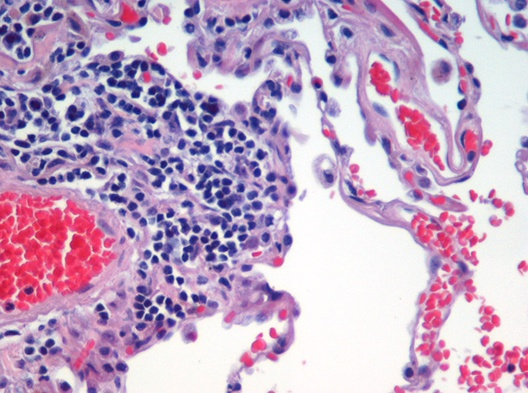
\includegraphics[width=7cm]{images/example.jpg}

The hematoxylin stains cell nuclei blue whereas eosin
stains the extracellular matrix pink, with other structures taking on
different shades, hues and combinations of these colors. The stain shows
the general layout and distribution of cells and provides a general
overview of a tissue sample's structure. It is the most widely used stain
in medical diagnosis. When a pathologist looks at a biopsy of a suspected
cancer, the histological section is likely to be stained with H\&E.

Collagen is one particular component of a tissue. It is a protein located
in the extracellular matrix, which becomes pink after the H\&E staining.
It is believed that the metastatic tumor cells interact with oriented
collagen fibers to invade the blood vessels. A specific Tumor Associated
Collagen Signature 3 (TAC-3) is defined to emphasise this interaction. Image
is considered to be TAC-3 positive if it contains many straight collagen
fibers aligned normally to the epithelial cells boundary regions: \\

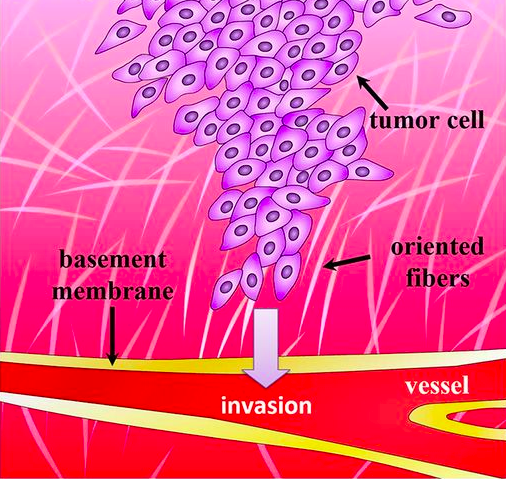
\includegraphics[width=7cm]{images/tac3.png}

Thus, collagen fibers organisation in the tissue could be used as a biomarker
to diagnose the patients cancer severity. This project aims to automate
collagen as a biomarker extraction and assesment procedures.

\section{Collagen Extraction}

The first step in this project is to take the H\&E stained image containing
all tissue components and extract only the shape of a collagen present
in the image. This is known as the image segmentation problem. In this case
a pixel representing the collagen will be labelled as a foreground, whereas any
other pixel will be labelled as a background. Machine learning was used
to solve this problem. A model is created and provided with the training data.
The model learns to separate pixels into collagen and background classes
and can be applied to unseen images.

The training data was provided by the National Center of Pathology, Vilnius.
Large H\&E images were tiled into $256 \cdot 256$ tiles and for each tile
a collagen mask was manually extracted: \\

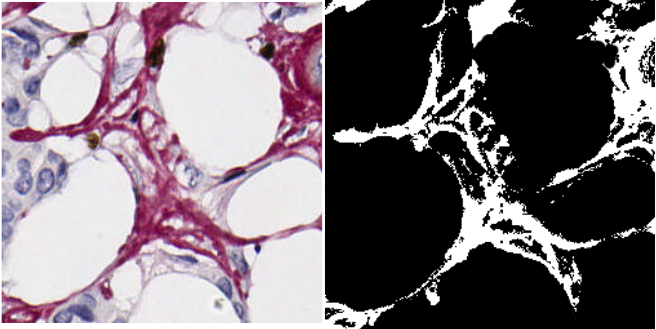
\includegraphics[width=7cm]{images/pair.png}

In total 43 image-mask pairs were used to train the model. A convolutional neural network U-net was chosen as a model: \\

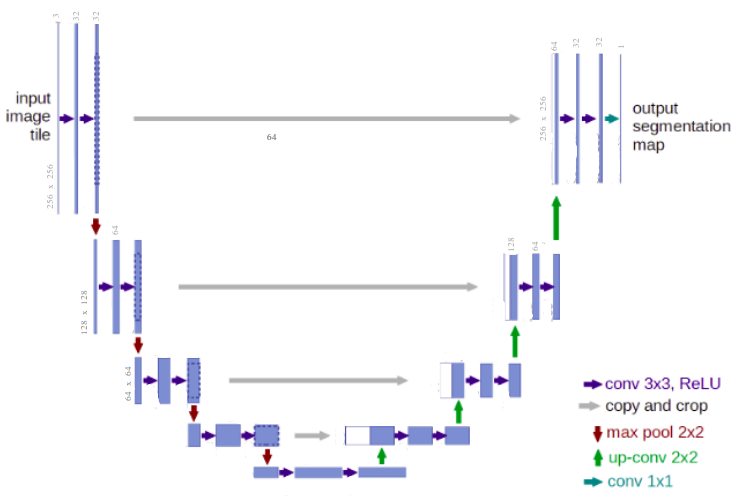
\includegraphics[width=\textwidth]{images/unet.png}

The model takes a full $256 \cdot 256$ (x3 for each of the RGB colour)
image as an input and performs a few downsampling procedures to infer the
deep features from the image. Each downsampled layer is then upsampled and
connected to the layer above to apply the inferred features on the image.
Eventually the model predicts the $256 \cdot 256$ mask.

The neural network was trained on the 43 image-mask pairs using the
cross-validation technique. Binary crossentropy was used as a loss function.
Accuracy (i.e. proportion of correct foreground / background pixels) metric
was used to test the model. All code was written in python using Keras
neural network API. After the model was trained, it was applied on a new
larger scale image to test its validity. The larger image was divided
into $256 \cdot 256$ tiles and the model was applied to each tile to extract
a collagen mask. The extracted masks were then merged into a large mask: \\

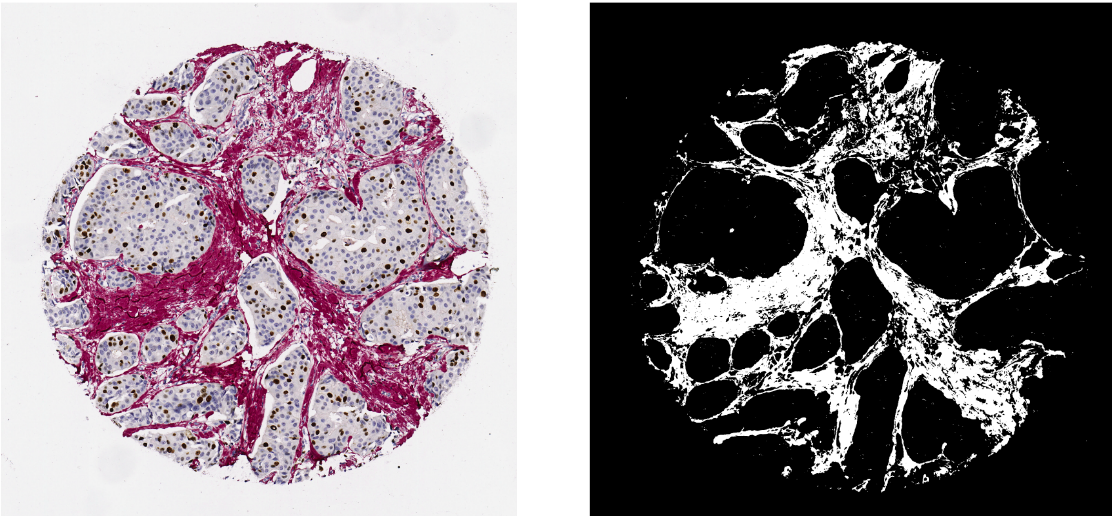
\includegraphics[width=\textwidth]{images/test.png}

\section{Features Generation}


After the collagen is extracted, the next step is to analyse it and compute
features that can allow to predict the patients diagnosis.



\end{document}
